\chapter{Plasmonic Nanomaterials}\label{sec:background:Plasmonics}
Recent advances in the fabrication of nano-scale, tailor-designed structures have allowed the exploration of novel optical effects arising from the interaction between light and nanomaterials. Perhaps most commonly exploited are plasmonic materials: metallic structures within a dielectric environment whose optical properties are affected not only by material choice, but also their structural geometry. 
The general response of a metal surface to incident light can be modelled in terms of plasma oscillations. By treating the metal as a free-electron gas (plasma) surrounding a lattice of positive charges, the electromagnetic response can be described by the motion of this plasma in response to external electromagnetic fields. 
At a metal-dielectric interface, incident light can drive electron-density waves that propagate along the metal surface. The coupled electromagnetic radiation and electron-density waves are known as surface plasmon polaritons (SPPs), and will propagate along the metal-dielectric interface, with an exponentially decaying intensity normal to the surface. 

\begin{figure}[htb!]
    \centering
    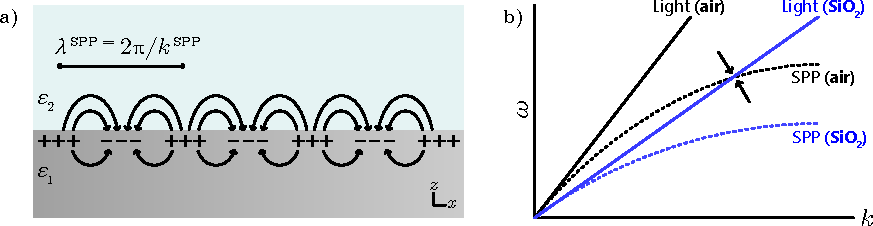
\includegraphics[scale=1.0]{./figures/background/plasmonics/spp.pdf}
    \caption{\label{fig:background:Plasmonics:SPP} \textbf{a)} Schematic of a surface plasmon polariton, of wavevector $k^{SPP}$, at a metal-dielectric interface. Charge density waves form in the metal surface, leading to surface-localised electromagnetic fields at the dielectric interface. \textbf{b)} Representative dispersion curves for surface plasmon polaritons and light at the interface of air or SiO$_2$. For any particular interface, SPPs cannot be excited by light impinging from the dielectric at that interface. Light propagating through glass can however be phase-matched to a SPP at a metal-air interface, for example. The momentum-matching point is illustrated with arrows. }
\end{figure}

We consider an interface between a metal and a dielectric, of permittivities $\varepsilon_1$ and $\varepsilon_2$ respectively (figure~\ref{fig:background:Plasmonics:SPP}a). The metal necessarily has permittivity ${\mathop{\rm Re}\nolimits}(\varepsilon_1)<0$. Excitation of SPPs require the real parts of $\varepsilon_1$ and $\varepsilon_2$ to be of opposite sign, that is, the interface is between a conductor and an insulator. In this configuration, the dispersion relation for a surface plasmon polariton propagating in the $x$ direction, oscillating at frequency $\omega$, is given by equation~\ref{eq:Plasmonics:SPPdispersion}~\cite[\S 2.2]{Maier2007}. 
\begin{equation}\label{eq:Plasmonics:SPPdispersion}
    k^{SPP}_{x} = k_0 \sqrt{\frac{\varepsilon_{1}\varepsilon_{2}}{\varepsilon_{1}+\varepsilon_{2}}} = \frac{\omega}{c} \sqrt{\frac{\varepsilon_{1}\varepsilon_{2}}{\varepsilon_{1}+\varepsilon_{2}}}
\end{equation}
For light incident on the interface via the dielectric described by $\varepsilon_2$, the optical dispersion relation $k_0 = \omega / c = \omega \sqrt{\mu_0 \varepsilon_2}$ shows that the optical momentum in the direction of SPP propagation will always be lower than that of the SPP (figure~\ref{fig:background:Plasmonics:SPP}b). Conservation of momentum must be considered when optically exciting surface plasmon polaritons, and so SPPs cannot be excited by light incident from the same dielectric as at the metal interface. Various experimental configurations have been demonstrated to allow the excitation of SPPs with optical radiation~\cite{Maier2007, Roh2011}, most commonly the Kretschmann and Otto geometries. These involve exciting a SPP at a metal-dielectric interface with light propagating through a different dielectric, interacting at an adjacent interface. In order for momentum matching to be properly realised, the projection of $k_0$ onto the axis of SPP propagation must match, and so depends strongly on the angle of optical incidence. Importantly for many applications, this angle is highly sensitive to changes in the dielectric environment. This allows the characterisation molecules attached to the metal surface by scanning the angle of incidence and observing induced shifts, leading to applications in molecular sensing and characterisation~\cite{Roh2011}.

In this work, we make use of plasmonic structure with characteristic dimensions comparable to, or smaller than, the wavelength of light in order to alleviate the momentum matching conditions. In these cases, the surface plasmons are confined to the nanoparticle surface, and are known as localised surface plasmons.


\section{Localised Surface Plasmons}\label{sec:background:Plasmonics:Metamaterials}

For small diameter $d \ll \lambda$ metallic nanoparticles, the phase of an oscillating electromagnetic field can be assumed constant over the particle, known as the ``quasi-static approximation''. In this approximation, the electron gas is driven to coherently oscillate at the particle surface. The lowest-order response of the particle to incident light can thus be described by an induced dipole moment $\bf{\tilde p}$, much like the simple Lorentz oscillator in section~\ref{sec:background:NonlinearOptics:lorentz} (figure~\ref{fig:background:Plasmonics:LSP}a).
For a metallic nanoparticle of permittivity $\varepsilon_1$ surrounded by a dielectric of permittivity $\varepsilon_2$, the induced dipole moment is described by equation~\ref{eq:Plasmonics:LSPdipole}. 
\begin{equation}\label{eq:Plasmonics:LSPdipole}
    {\bf{\tilde p}} = {\bf{\tilde \alpha }}{\bf{\tilde E}}
\end{equation}
As in section~\ref{sec:background:Chirality:opticalchirality}, $\bf{\tilde \alpha }$ describes the complex electric polarisability of the particle, and depends strongly on the nanoparticle material, geometry, and the permittivity of the surrounding medium.
Importantly, the induced dipolar plasmon mode is non-propagating, and so the momentum-matching requirements for exciting propagating surface plasmon polaritons are alleviated. The localised surface plasmon can be coherently excited by any oscillating electromagnetic field, and will reach a maximum excitation efficiency at a particular resonant frequency determined by the effective polarisability ${\tilde \alpha }(\omega)$ of the nanoparticle.
Analytical expressions for ${\tilde \alpha }(\omega)$ are well established for simple spherical nanoparticles of radius $a \ll \lambda$ and permittivity $\varepsilon(\omega)$~\cite{Maier2007, Collins2017}, given by equation~\ref{eq:Plasmonics:LSPalphaSphere}. 
\begin{equation}\label{eq:Plasmonics:LSPalphaSphere}
    {\tilde \alpha } = 4\pi a^3 \frac{\varepsilon (\omega) - \varepsilon_2 (\omega)}{\varepsilon (\omega) + 2\varepsilon_2 (\omega)}
\end{equation}
At the point where $\lvert \varepsilon (\omega) + 2\varepsilon_2 (\omega) \rvert$ is at it's minimum, i.e $\varepsilon (\omega) = -2\varepsilon_2 (\omega)$, the polarisability is maximally enhanced, determining the resonant frequency of the localised surface plasmon. However, in many systems the nanoparticle geometry is significantly more complex, and the LSP resonance cannot be determined analytically. Regardless of the particle geometry however, a particular resonant frequency will exist at which the plasmonic nanoparticle will resonantly scatter. Similar to surface plasmon polaritons, the sensitivity of the resonant frequency to the dielectric environment makes spectral analysis of the plasmonic scattering a sensitive technique for characterising nearby molecules, and has also gained popularity in molecular sensing applications~\cite{Petryayeva2011a, Polavarapu2014, Cheng2015}.


\begin{figure}[htb!]
    \centering
    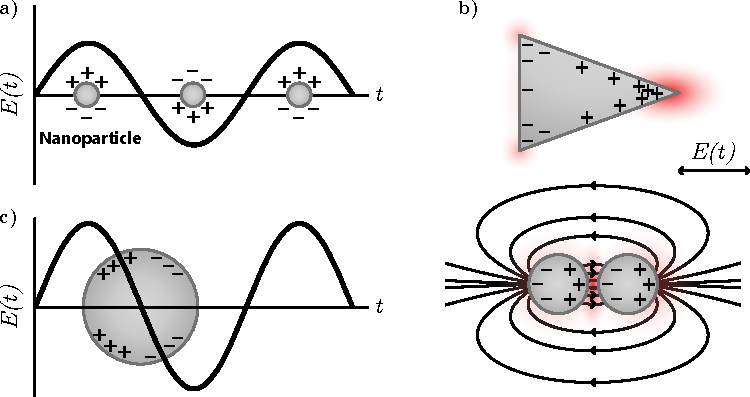
\includegraphics[scale=1.0]{./figures/background/plasmonics/lsp.pdf}
    \caption{\label{fig:background:Plasmonics:LSP} \textbf{a)} For sub-wavelength metallic nanoparticles, charge is coherently driven at the surface, and the particle can be approximated to an oscillating dipole. \textbf{b)} A pair of nanoparticles separated by some small distance will couple via the near-field, and function as a single dipole with an additional capacitance from the gap. Charge is efficiently confined to the inner surface, resulting in an enhanced electric field intensity between the two particles.}
\end{figure}


\subsection{Electromagnetic Field Confinement}\label{sec:Plasmonics:confinement}

An effect crucial to this work, and indeed the field of nanophotonics generally, is the ability for plasmonic nanoparticles to confine electromagnetic fields into sub-wavelength ``hotspots''. This confinement results in two useful properties: the field is highly localised to small regions of space, allowing targeting of electromagnetic interactions to regions below the diffraction limit, and correspondingly, the field intensity is enhanced within these regions. The precise mechanism of field confinement depends largely on the system being considered, however perhaps the simplest contribution is from the localised surface plasmon resonance. 
When a metallic nanoparticle is excited close to a plasmon resonance, the induced dipole oscillates at its maximum amplitude. This results in a resonant scattering of light, leading to locally enhanced electromagnetic fields around the particle. For sub-wavelength nanoparticles, this allows for sub-wavelength field confinement: The localised surface plasmon mode volume is limited by the particles dimensions, and the local electromagnetic field is determined by the, now tightly confined, surface plasmon oscillation. Coupling this surface plasmon mode to incident light results in an enhanced local electromagnetic field at the particle surface. Like the LSP resonance itself, the enhancement factor (the ratio of the field amplitude at the particle surface, and without the particle present) at resonance strongly depends on the particle material, geometry, and surroundings~\cite{Dynich2009, Tanabe2008}.

Aside from enhanced near-fields at the plasmon resonance, geometric effects can lead to even greater levels of field confinement, with correspondingly high intensity enhancements. Broadly, any effect that confines charge to a region of space within a conductor will lead to enhanced electromagnetic fields at the conductor surface. 
An important contribution in plasmonic nanostructures can come from the lightning-rod effect. In the context of electrostatics, the lightning-rod effect describes the confinement of electric fields at sharp gradients of conducting structures, such as corners or tapered tips. Charge is confined more efficiently to regions of sharp surface gradients on a charged conductor, and so the electric field lines at the surface of the conductor will generally be localised around these sharp features. In spherical nanoparticles, the curvature of the sphere results in charge confinement at the surfaces along the axis of excitation polarisation, resulting in greater field confinement along this direction~\cite{Tanabe2008}. However, nanostructure geometries with sharper features greatly increase the field enhancement associated with the lightning-rod effect, localising the field strongly at sharp corners and edges~\cite{Dreaden2011, Lee2010, Valev2012d}.

Another contribution to field enhancement associated with charge confinement is from coupling between plasmonic nanostructures. A simple example is a pair of sub-wavelength nanoparticles, separated by a distance $d \ll \lambda$. This system behaves as a pair of point dipoles interacting via the near-field (figure~\ref{fig:background:Plasmonics:LSP}b). In the limit of small separation $d$, the coupled system will radiate as a dipole, and resonantly scatter when excited by light at it's resonant frequency. When driven by a field polarised along the chain axis, the gap between particles introduces a capacitance dependent on particle geometry and separation. This capacitance red-shifts the resonant frequency of the longitudinal hybridised plasmon mode along that axis. When driven by light polarized perpendicular to the chain axis, a transverse hybridised plasmon mode is excited, with lower inter-particle capacitance, blue-shifting the resonant frequency. Crucially, the capacitance of the inter-particle gap results in the confinement of charge on the inner surfaces of the particles. The confinement of charge directly leads to confinement of the electromagnetic fields in the region between particles. Both the inter-particle field confinement, and associated shifts in the LSP resonance have been studied experimentally and theoretically for long chains of nanoparticles~\cite{Krenn1999, Krenn1999a}, pairs of nanoparticles~\cite{Huang2016}, and periodic nanostructure arrays~\cite{Lee2016, Valev2011b, Valev2012a}.

The ability to strongly confine electromagnetic fields has found a wide range of applications, of particular note in surface-enhanced Raman scattering (SERS). Raman scattering experiments typically probe molecular transitions by spectroscopically analysing light inelastically scattered from a molecule. Spectral shifts in the scattered light correspond to the energy of molecular transitions, acting as a probe for substance composition. However, the probability of inelastic scattering is low compared to elastic scattering, and thus Raman scattering it typically a very weak effect. In SERS experiments, molecular samples are bound close to a nanostructured metal surface. Incident light resonantly excites surface plasmons in the metallic structures, leading to an enhanced near-field at the metal surface. The enhanced near-field scatters from the molecular sample, and the plasmonic nanostructures can then function as resonant transmitting antennae for the scattered light, providing a second source of enhancement. The combination of these two sources of enhancement lead to a potential enhancement in the overall detected Raman scattering signal of $10^{10}$~\cite{Fromm2006}. Although the precise limitations of SERS are debated~\cite{LeRu2007}, enhancements of several orders of magnitude have nevertheless been experimentally demonstrated using coupled spherical nanoparticles~\cite{Talley2005}, bowtie antennae (making use of the lightning-rod enhancement)~\cite{Fromm2006}, and roughened metal surface, showing sensitivity down to single-molecule detection~\cite{Blackie2009}. Plasmonic field confinement has also found applications in sub-wavelength imaging~\cite{Huang2010a}, photodetection~\cite{Ishi2005}, and scanning near-field optical microscopy (SNOM)~\cite{Wenzel2008} by making use of sub-wavelength resonant antennae.

\subsection{Enhanced Second-Harmonic Generation}\label{sec:background:NonlinearOptics:plasmonic}
In section~\ref{sec:background:NonlinearOptics} we established that the amplitude of second-harmonic generation varies with $E^2$, and correspondingly the SHG intensity follows $E^4$, where $E$ is the amplitude of incident light. This sensitivity to the driving field amplitude allows SHG to be greatly enhanced in regions of strong local fields, such as plasmonically confined hotspots. The requirement for inversion asymmetry generally prevents SHG from the bulk of metallic structures. However, the metallic surface interface breaks centrosymmetry allowing surface SHG. Surface plasmons then confine the incident light to the nanoparticle surface, increasing the surface SHG intensity. 
The first experimental demonstration of SHG enhancement from surface plasmons reported a $30\times$ increase in SHG intensity~\cite{Simon1974}. Since then, orders of magnitude SHG enhancement have been demonstrated from a range of nanoparticle geometries including coupled nanoparticles~\cite{Yildiz2015}, individual particles within plasmonic cavities~\cite{Xiong2016}, periodic nanostructure arrays~\cite{Valev2011b}, and metallic nanoshells~\cite{Pu2010}. Enhanced SHG has also been deployed as an experimental probe for measuring confined fields between a plasmonic nanoparticle and metallic surface, with applications in sub-wavelength spatial measurements~\cite{Shen2015a}. 

Importantly, plasmon enhanced SHG has been applied to molecular sensing platforms. As discussed in section~\ref{sec:background:NonlinearOptics:chirality}, second-harmonic generation has long been used in chemical characterisation~\cite{Chowdhury2016}, molecular sensing~\cite{Tran2017}, and disease diagnosis~\cite{Campagnola2011} owing to its symmetry sensitivity, both providing structural information~\cite{Gott2001} and reducing background signal from SHG-forbidding structures~\cite{Wanapun2010}. 
However, second-harmonic signals from small quantities of molecules tend to be weak. By making use of both the intensity enhancement~\cite{Kai2007, Wang2018} and sensitivity to changes in the nanostructures surrounding medium~\cite{Ghirardini2018}, plasmonic nanomaterials have provided a platform to greatly improve the sensitivity of sensing techniques.
Similarly, we discussed in section~\ref{sec:background:NonlinearOptics:chirality} the use of second-harmonic generation as an ideal probe for structural chirality, due to the intrinsic lack of centrosymmetry of chiral structure. It has been shown that, in large part due to the enhancement in SHG intensity from local field confinement, plasmonic nanomaterials can lead to increased sensitivity of nonlinear optical activity measurements~\cite{Valev2012a, Chen2016, Huttunen2011}.


\subsection{Enhanced Chiral-Optical Interactions} \label{sec:background:Plasmonics:chiralPlasmonics}
\begin{itemize}
    \item Freedom of fabrication techniques allow symmetries to be explored.
    \begin{itemize}
        \item Helically arranged nanoparticles using DNA~\cite{Shen2012}
        \item Using molecules as ligands to create chiral arrangements of gold clusters~\cite{Knoppe2012a}, exhibiting large experimentally measured SHG~\cite{Knoppe2012}
        \item Method for fabrication of water-soluble chiral silver nanoparticles, exhibiting strong CD signal~\cite{Farrag2016}

    \end{itemize}
    \item Second-order nonlinear processes, which already enhance chiroptical measurements, can themselves be enhanced as described in section~\ref{sec:Plasmonics:confinement}.

    \item Achiral example: Matching the plasmon resonance frequency of a metamaterial to the vibrational fingerprint of a molecule to be analysed. The enhanced local fields allowed the demonstration fo 5 orders of magnitude enhancement in the molecular absorption, for applications in extremely low concentration molecular detection~\cite{Cheng2015}
    \item Enhanced circular dichroism of a molecule between two spherical nanoparticles (in the region of maximally localised field), away from the molecular resonance. This demonstrates a transfer of chirality from the molecule to the plasmon resonance~\cite{Zhang2013}
    \item Two monolayers of chiral molecules around achiral gold nanostructures exhibit enhanced CD, not observable without the plasmonic enhancement~\cite{Maoz2013}
    \item Two orders of magnitude enhanced CD of molecules at local field hotspots of gold nanoparticle chains, again demonstrating transfer of molecular chirality to the plasmon resonance~\cite{Wang2014c}
    \item Another example of plasmonic nanoparticles introducing additional CD contributions around the plasmon resonance, suggesting transfer of chirality~\cite{DiGregorio2015}

    \item Attomolar detection of DNA through DNA-linked gold nanorods~\cite{Ma2013b}

    \item Introduce: Aside from enhancements from coupling to intense localised field hotspots, plasmonic nanomaterials have been demonstrated to exhibit regions of superchiral local fields.
\end{itemize}

\subsubsection{Superchiral Fields from Plasmonic Nanostructures} \label{sec:background:Plasmonics:superchiral}
\begin{itemize}
    \item Seminal paper, ``Ultrasensitive detection and characterization of biomolecules using superchiral fields''~\cite{Hendry2010}. ``Here, we show that superchiral electromagnetic fields, generated by the optical excitation of plasmonic planar chiral metamaterials, are highly sensitive probes of chiral supramolecular structure.''
    \item Investigation, via simulations, of the superchiral near fields generated from a range of both planar and 3-dimensional chiral plasmonic nanostructures~\cite{Schaferling2012}
    \item Achiral plasmonic nanostructures pumped with linearly polarised (achiral) light, showing that although the optical chirality of the near field integrated over all space is $0$, regions within the nanostructure's near-field volume exhibit high optical chirality~\cite{Schaferling2012a, Davis2013}. It is proposed that by masking regions of the structure exhibiting one handedness of optical chirality, a non-zero macroscopic chiroptical response can be obtained within this regime~\cite{Schaferling2012a}.
    \item Experimental demonstration of disposable plasmonic metasurfaces fabricated on a polymer substrate. The optical chirality of the near-field can be tuned by changing relatively simple geometric properties such as the nanostructure film thickness~\cite{Karimullah2015}. These metasurfaces were later used to demonstrate ``superchiral polarimetry'', measuring the optical rotatory dispersion of the metasurface in the presence of proteins, which shift the plasmon resonance depending on the protein structure. This shift also depends on the handedness of the underlying metasurface, and so is measured as an enhanced chiral asymmetry in the ORD spectra, providing comprehensive structural information~\cite{Tullius2015}.
    \item Novel fabrication techniques have also been demonstrated to allow ultra-broadband generation of superchiral fields from chiral metamaterials, leading to both large circular dichroism and optical rotation at optical wavelengths~\cite{Hou2016}

    \item Superchiral fields have also been shown to contribute to enhanced second-harmonic optical activity. Both SHG and optical activity have components proportional to electric field gradients, and so regions of high optical chirality are expected to directly enhance SHG, and corresponding nonlinear chiroptical effects~\cite{Valev2014}.
\end{itemize}

\section{Metamaterials}
By fabricating arrays of sub-wavelength plasmonic nanostructures, it is possible to create artificial ``metamaterials''. In arrays of nanoparticles supporting localised surface plasmons, the system can be modelled as an array of oscillators with effective polarisabilities. The macroscopic behaviour of the array can then be described as an effective medium, with a susceptibility describing its optical response as in section~\ref{sec:background:NonlinearOptics:susceptibility}. Now, the macroscopic optical properties of the metamaterial are strongly related to the geometry of the individual nanoparticle inclusions, offering unprecedented flexibility to design materials exhibiting optical properties never observed in nature. An often cited example of this is the possibility of a perfect optical lens formed from a metamaterial with negative refractive index, as proposed by Veselago~\cite{Veselago1968}, and later expanded on by Pendry~\cite{Pendry2000}. Further work has proposed the use of metamaterials for photonic devices such as perfect reflectors~\cite{Moitra2015}, polarisation optics~\cite{Cong2015}, and chiral-optical devices, as discussed in section~\ref{sec:background:Plasmonics:chiralPlasmonics}.

Of particular interest in this work are meta-\textit{surfaces}. These consist of plasmonic nanostructures patterned onto the surface of a dielectric substrate creating a quasi-2-dimensional metamaterial. Whereas 3D metamaterials typically exhibit novel optical properties from light propagating through the bulk, 2D metamaterials act to manipulate the wavefront of incident fields at the surface~\cite{Meinzer2014}. This has potential applications in new ultra-thin optical components. Since traditional optics generally rely on small effects building up throughout propagation through the material, they are generally much thicker than a metasurface designed to exhibit the same total effect on the wavefront~\cite[\S 3]{Yao2014}. Additionally, they are ideal for studying plasmon enhanced SHG, since the primary contribution to SHG comes from the material surface anyway, with little to no bulk contribution. 

By treating a plasmonic nanostructure array as an effective medium, a macroscopic description of the optical response can be employed, as in chapters~\ref{sec:background:Chirality} and~\ref{sec:background:NonlinearOptics}. This allows the nanomaterial to be characterised by macroscopic parameters such as effective susceptibility, refractive index, and structural chirality. These can be quantified by measuring macroscopic effects such as circular dichroism and optical rotation of reflected light, or nonlinear chiroptical counterparts SHG-CID and SHG-OR. The work in chapters~\ref{sec:results:OAinPlanarNanohelices} and~\ref{sec:results:HRS} in particular treat our nanostructure samples as an effective medium, with macroscopic properties.

\section{Beyond the Quasi-Static Approximation}
\begin{itemize}
    \item Intermediate regime of nanostructures, beyond the quasi-static approximation. Structure dimensions are close to, or larger than, the wavelength.
    \item The near-field optical behaviour in this regime can be understood in terms of higher order current density modes.
    \begin{itemize}
        \item The geometry of the metallic surface will permit a set of plasmon modes.
        \item Higher order plasmon modes can be excited across the surface of the structure.
        \item These modes are non-propagating standing waves, and have zero net momentum. Thus, even in this intermediate regime momentum matching is not a requirement to excite surface plasmons.
    \end{itemize}
    \item Literature review
    \begin{itemize}
        \item Zheng's work demonstrated that the plasmonic response of metallic nanostructures in this intermediate regime can be decomposed into a set of current density eigenmodes~\cite{Zheng2012}. This work was extended to collections of coupled nanostructures~\cite{Zheng2013}. 
        \item The optical response can be further understood by applying group theory to the plasmonic eigenmode set~\cite{Zheng2015}, allowing the current density modes to be grouped by the optical polarisation states that exclusively excite them.
    \end{itemize}

    The work in chapter~\ref{sec:results:EnantiomorphingChiralCrosses} considers nanostructures within this regime, where a full modal analysis must be employed to properly describe the optical properties of the material surface.
\end{itemize}


\section{Conclusions}

By modelling the optical response of a metal as an electron plasma surrounding a lattice of positive charge, we have shown that metallic nanoparticles significantly smaller than the wavelength of light will behave as an oscillating electric dipole. This coherently driven electron oscillation is known as a localised surface plasmon (LSP). The restoring force on the LSP, and hence resonant frequency of the dipole oscillation, will depend not only on the nanoparticle material, but also the geometry of the nanoparticle itself. This allows the optical properties of nanoparticles to be tailored by changing only the dimensions and shape of the particle. Additionally, the surrounding medium will affect the resonant properties of the LSP, and so LSP resonances can be used for the sensitive characterisation of media surrounding, or attached to the surface of, metallic nanoparticles.
This surface sensitivity is further enhanced by the remarkable ability for plasmonic nanoparticles to locally confine electromagnetic fields. Three key contributions to field confinement are discussed. When driven at resonance, the plasmonic nanoparticle will resonantly scatter light, increasing the electromagnetic intensity surrounding the nanoparticle. Additionally, nanoparticles with sharp geometric features will confine charge in these regions. This charge confinement directly leads to the confinement of electric fields at the surface, analogous to the lightning rod effect in electrostatics. Finally, charge confinement is also induced when a multiple nanoparticles are coupled via the near-field. When a pair of plasmonic nanoparticles are separated by a dielectric medium, the capacitance of the gap confines charge at the inner surface, leading to strong field confinement in the space between the nanoparticles, and a shift in the LSP resonance.
Crucially to this work, these confined electromagnetic fields have been shown to enhance both chiroptical interactions with structures surrounding the confined fields, and nonlinear emission due to the strong intensity dependence of higher-order nonlinearity. 
By fabricating periodic arrays of sub-wavelength nanostructures, artificial metamaterials can be developed. Since the structure can be modelled as an array of coupled electric dipoles, it can be macroscopically described as an effective medium. The macroscopic optical properties will strongly depend on the nanostructure geometry, material, and surroundings, allowing for plasmonic enhancements to be utilised on a macroscopic scale.
The unique ability to design metamaterials of arbitrary geometry allowed the study of chiroptical effects as a sample transitions from one handedness to the other (section~\ref{sec:results:EnantiomorphingChiralCrosses}), of isolating the structural chirality of a highly anisotropic metamaterial (section~\ref{sec:results:OAinPlanarNanohelices}), and finally the first demonstration of optical activity in hyper-Rayleigh scattering, using chiral nanoparticles isotropically suspended in solution (section~\ref{sec:results:HRS}). In these works, the enhancement of second-harmonic generation from local field enhancement, chiroptical interactions from plasmonically enhanced chiral near-fields, and the combined enhancement available from nonlinear chiroptical measurements, have all been used to develop new experimental techniques for the detection and characterisation of chiral metamaterials.
